\documentclass[xcolor=dvipsnames]{beamer} 
\usecolortheme[named=Gray]{structure} 
\setbeamertemplate{blocks}[shadow=true] 
\usepackage{ucs}
\usepackage{wasysym}
\usepackage[utf8x]{inputenc}
%\input beamerthemeumbc4.sty
%\usepackage{beamerthemeumbc4}
\useoutertheme{shadow}
%\usetheme{Madrid} % My favorite!
%\usetheme{Boadilla} % Pretty neat, soft color.
%\usetheme{umbc4}
\usetheme{Ilmenau}
%\usetheme{Amsterdam}
%\usetheme{CambridgeUS}
%\usetheme{Berlin}
%\usetheme{Warsaw}
%\usetheme{Bergen} % This template has nagivation on the left
%\usetheme{Frankfurt} % Similar to the default 
%with an extra region at the top.
%\usetheme{Darmstadt} % not so good
\usecolortheme{beaver} % Simple and clean template
% Uncomment the following line if you want %
% page numbers and using Warsaw theme%
% \setbeamertemplate{footline}[page number]
%\setbeamercovered{transparent}
\setbeamercovered{invisible}
% Get rid of navigation
\setbeamertemplate{navigation symbols}{} 
% To remove the navigation symbols from 
% the bottom of slides%
\setbeamertemplate{navigation symbols}{} 
%
\usepackage{graphicx}
%\usepackage{bm}         % For typesetting bold math (not \mathbold)
%\logo{\includegraphics[height=0.6cm]{debian-text.eps}}
%
\title[A universal project, with a global community]{The Debian Project}
\author{Victor Ni\c{t}u}
\institute[Ceata, Debian Romania]
{
Ceata Foundation\\Debian/RO Community\\
\medskip
{\emph{victor@debian-linux.ro}}
}
\date{June 11, 2012\\Bucharest, Romania}
% \today will show current date. 
% Alternatively, you can specify a date.
%
\begin{document}
%
\begin{frame}
\titlepage
\end{frame}
%
\begin{frame}
\frametitle{Summary}
\begin{itemize}
\item Introduction in Debian philosophy
\item Specific concepts
\item Statistics
\item The global community
\item The Romanian community
\item How to become a member? Why?
\end{itemize}
\end{frame}
%
\section{Debian Philosophy}
\begin{frame}
\frametitle{Concepts specific to Debian}
\begin{block}{}
\begin{itemize}
\item Not owned by a company
\item Ensuring freedom of ideas and included software
\item The biggest community-driven project
\item Universal - runs on many platforms
\item Accessible - optimized for users with physical disabilities
\end{itemize}
\end{block}
\end{frame}

\subsection{Freedom's documents}
\begin{frame}
\frametitle{Debian means Freedom}
\footnotesize{
\begin{thebibliography}{99}
 \bibitem[Label1]{key1} Debian Social Contract
 \newblock The essential document in the Debian - developers/users relationship
 \newblock \emph{Guarantees project's freedom, and its own persistence.}
 \bibitem[Label2]{key2} DFSG
 \newblock Debian Free Software Guidelines
 \newblock \emph{Extends Debian Social Contract by defining a set of rules to summarize free software concepts.}
\end{thebibliography}
}
\end{frame}
%

\begin{frame}
\frametitle{Debian means Freedom}
\begin{block}
{Indications extracted from the DFSG}
Free software characteristics:\\
\begin{itemize}
\item free redistribution
\item source code availability and inclusion
\item modification is allowed
\item eliminates any group / intent / user discrimination
\item ensures license keeping
\item license must be kept outside Debian, too
\end{itemize}
\end{block}
\begin{normalsize}
\hfill Licenses accepted as free: GPL, BSD, CC-BY-SA
\end{normalsize}
\end{frame}
%
\subsection{Public interest development}
\begin{frame}
\frametitle{Project structure}
\begin{block}
{}
Debian is a trademark of SPI (Software in Public Interest)
\end{block}
\begin{block}{}
His hierarchy and structure consists exclusively of project members
\end{block}
\begin{block}{}
There is a Project Leader, chosen by annual election, who publicly represents Debian interests
\end{block}
\begin{normalsize}\hfill
Any Debian Member can have an opinion on the project's evolution, this usually leading to a community-driven decision.
\end{normalsize}
  \raisebox{40mm}[0pt][0pt]{%
    \begin{pgfpicture}{-7mm}{30mm}{0mm}{0mm}
		
\includegraphics[height=1.75cm]{../images/zack.jpg}
    \end{pgfpicture}
  }
\end{frame}
%
\subsection{The universal operating system}
\begin{frame}
\frametitle{Availability and accessibility}
\begin{block}
{Hardware}
In order to run Debian, you only need a minimalistic hardware setup.
\end{block}
\begin{block}
{Architectures}
Debian can be installed on various environments, such as personal computers, laptops, mobile phones, servers, embedded devices and so on...
\end{block}
\begin{block}
{Ports}
Debian isn't built only around Linux kernel. We now have ports to Hurd and kFreeBSD kernel alternatives.
\end{block}
\end{frame}
%
\begin{frame}
\frametitle{Availability and accessibility}
\begin{block}
{Accessible}
Debian is configured out-of-the-box in order to be used by almost everybody.\\
\begin{itemize}
\item Very good support for Braille terminals
\item Nice integration of text-to-speech engine
\item Easy configuration method for the default console display, in order to set the default font family or size.
\item Natural detection of auxiliary hardware, such as peripherals, cards and drives.
\item Translated in over 50 languages.
\end{itemize}
\end{block}
\end{frame}

\section{Statistics}
\subsection{Debian on the map}
\begin{frame}
\frametitle{Some Debian numbers}
\begin{block}
{Developer-centric demographics}
\begin{itemize}
\item Finland is on the first place with the biggest active members percent, it currently have 21 active developers and a strong proportion of 4 / million inhabitants
\item \textbf{USA}, \textbf{Germany} and \textbf{France} are leading when it comes to total active developers, with \textbf{165}, \textbf{155}, respectively \textbf{94} DD/DM accounts.
\item Romania is on \textbf{46th} position, with 2 members, and only one active.
\end{itemize}
\end{block}
\begin{block}
{General stuff}
As a big total, we currently have developers from \textbf{59} countries.\\
At this moment, \textbf{920}, out of \textbf{1490} are active and bringing important contributions to the project.
\end{block}
\end{frame}

\subsection{Debian and other Linux distributions}
\begin{frame}
\frametitle{Debian and server applications}
  \raisebox{-40mm}[0pt][0pt]{%
    \begin{pgfpicture}{-10mm}{-2.5mm}{0mm}{0mm}
		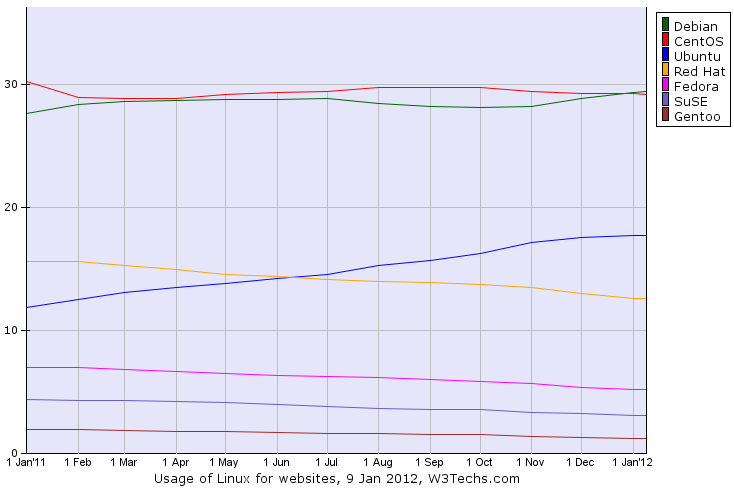
\includegraphics[height=6cm]{../images/debian-server.png}
    \end{pgfpicture}
  }
\end{frame}

\begin{frame}
\frametitle{Debian - genealogy}
  \raisebox{-40mm}[0pt][0pt]{%
    \begin{pgfpicture}{-65mm}{8mm}{0mm}{0mm}
		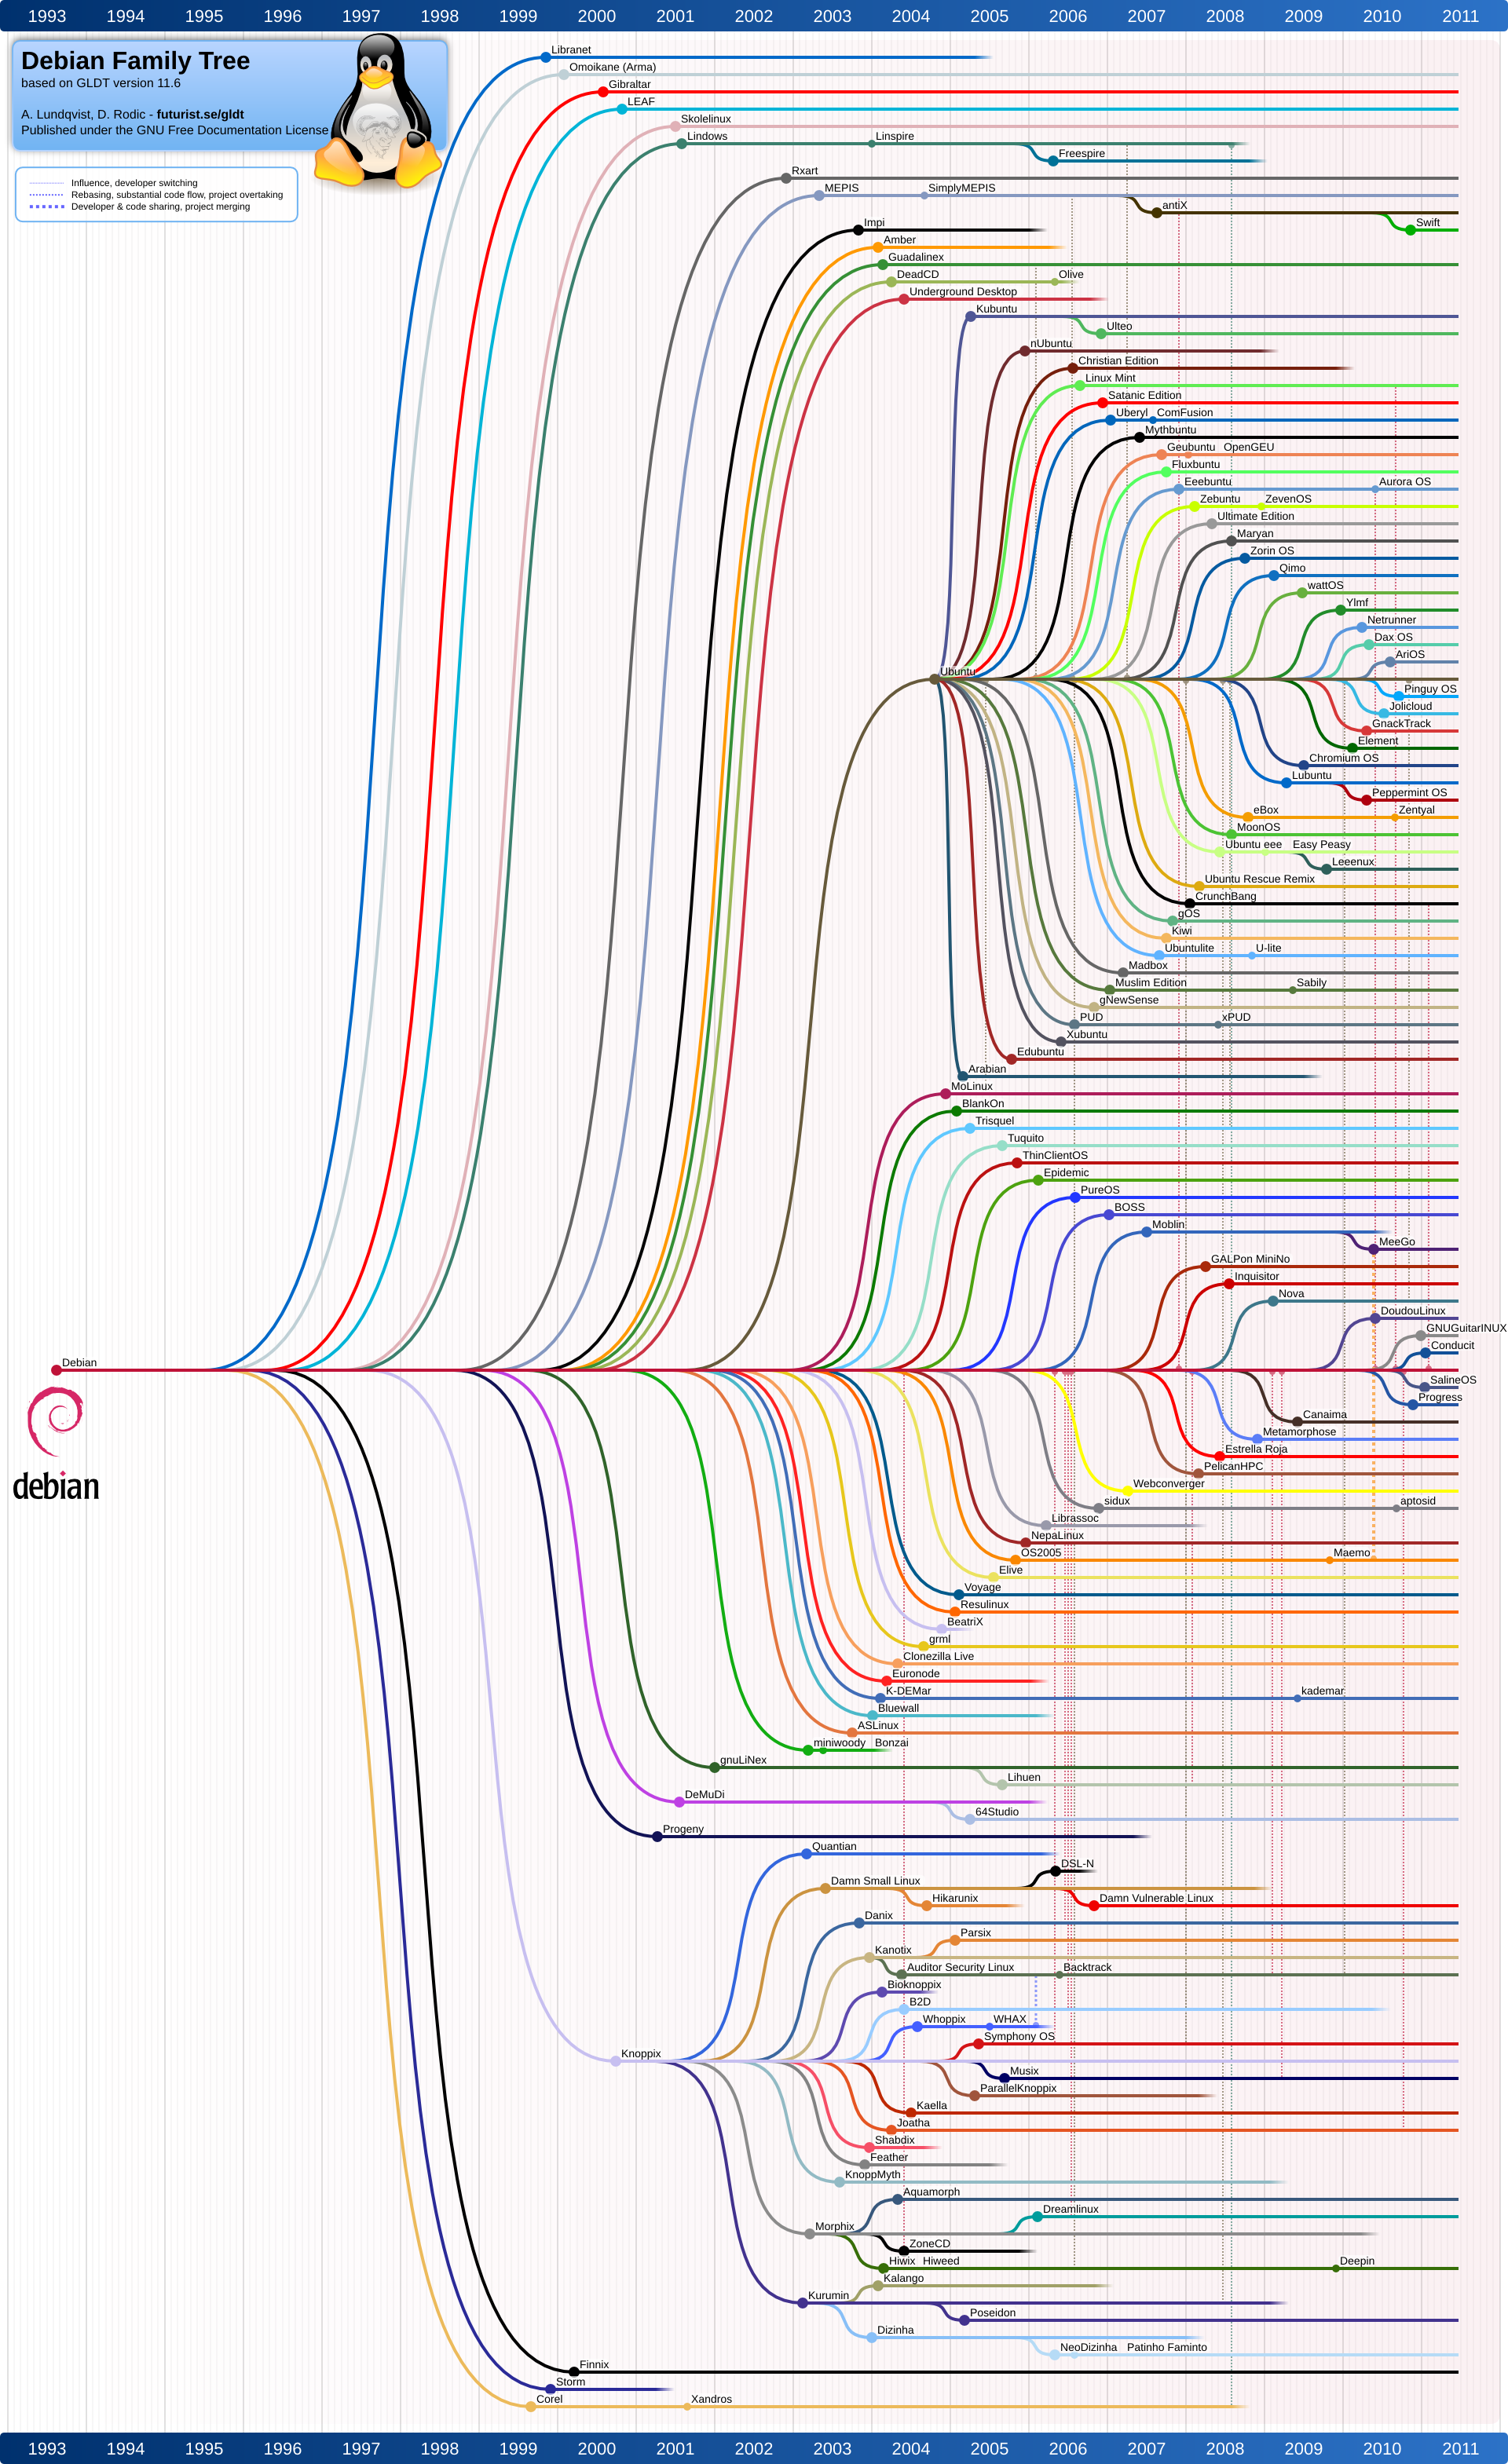
\includegraphics[height=6.5cm]{../images/debian-tree.png}
    \end{pgfpicture}
  }
	\begin{itemize}
		\item Ubuntu
		\item Linux Mint
		\item MeeGo
		\item Knoppix
		\item DSL (Damn Small Linux)
	\end{itemize}
\end{frame}

\section{News}
\begin{frame}
\frametitle{Debian 7.0 - Wheezy?}
\begin{block}
{When?}
\begin{small}
At the end of June 2012, Debian/testing will enter \emph{freeze}, while everybody will work intensively to fix the remaining RC bugs.\\
We expect a Wheezy release for the first half of 2013.
\end{small}
\end{block}
\end{frame}

\begin{frame}
\frametitle{Freeze}
  \raisebox{-40mm}[0pt][0pt]{%
    \begin{pgfpicture}{-12.5mm}{0mm}{0mm}{0mm}
		
\includegraphics[height=7cm]{../images/freeze.png}
    \end{pgfpicture}
  }
\end{frame}

\subsection{Wheezy News}
\begin{frame}
\frametitle{What's new?}
\begin{block}
{Multi-arch}
The possibility to create packages for different architectures without actually needing to install / bootstrap them (dpkg/multiarch).
\end{block}
\begin{block}
{debian-installer accessibility}
Default support for WPA authentication\\
Native ARM support
\end{block}
\begin{block}
{Kernel update}
Debian GNU/Linux will run on top of a 3.x kernel.
\end{block}
\end{frame}


\section{Debian Community}
\begin{frame}
\frametitle{Debian Planet}
\begin{block}
{What's that? What's so special about it?}
\begin{itemize}
\item People from many different domains and activities
\item People who only meet rarely, and happily!
\item Activists in favor of software and general freedom
\item Journalists, engineers, passionate users, hackers or artists, they all work on the same big project
\end{itemize}
  \raisebox{0mm}[0mm][0pt]{%
    \begin{pgfpicture}{-50mm}{10mm}{0mm}{0mm}
		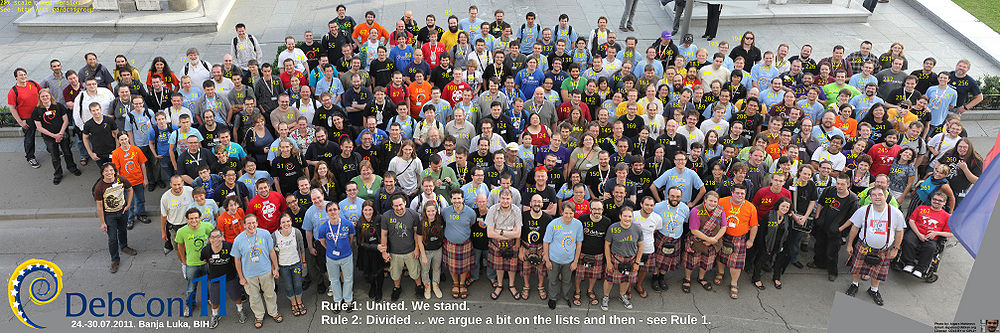
\includegraphics[height=2cm]{../images/debconf11.jpg}
    \end{pgfpicture}
  }
\end{block}
\end{frame}

\subsection{Why bother?}
\begin{frame}
\frametitle{Why? How? Me?!}
\begin{block}
{The Good}
\begin{itemize}
\item You can have an influence about where Debian is going
\item The opportunity to work with some brilliant people
\item Whatever you might do well, you can do it here too
\item Immediate recognition and feedback for your efforts
\item A very friendly environment
\end{itemize}
\end{block}
\begin{block}
{The Bad}
\begin{itemize}
\item Good decisions are usually coming slowly
\item Responsibility grows together with the amount of derivatives that might use your work
\item This global scatter can make online synchronization very difficult
\end{itemize}
\end{block}
\end{frame}

\subsection{Debian Romanian Community}
\begin{frame}
\frametitle{The debian-linux.ro story}
\begin{block}{}
...began in February 2011, with the help of ServerHost.\\
\hfill\\
What we've built so far:
\begin{itemize}
\item A web forum
\item An informative Debian website
\item The foundation for a local community
\end{itemize}
\end{block}
  \raisebox{0mm}[0mm][0pt]{%
    \begin{pgfpicture}{-75mm}{-8mm}{0mm}{0mm}
		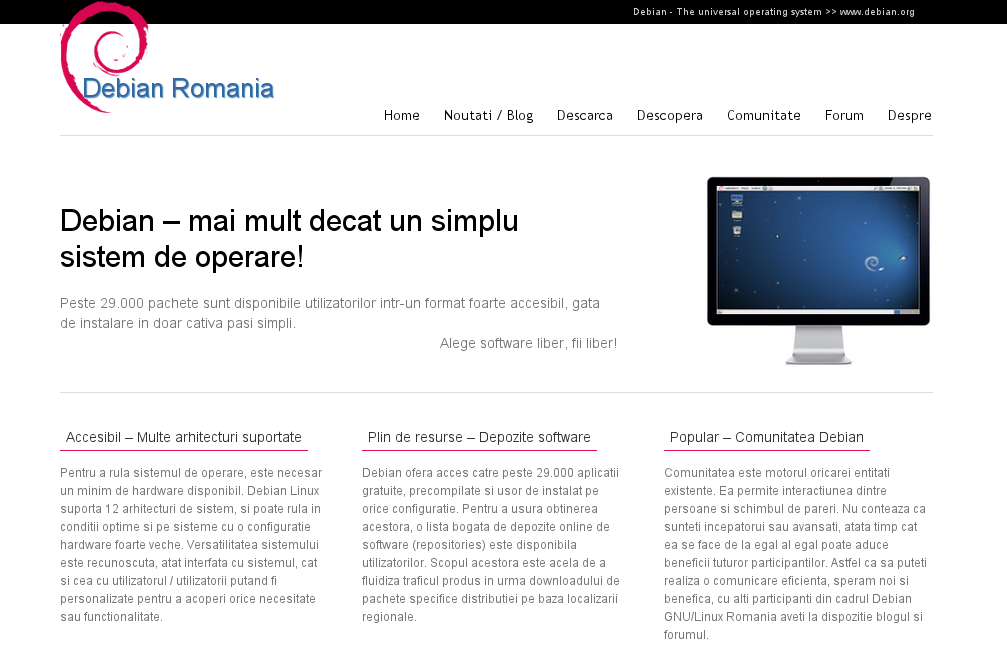
\includegraphics[height=2cm]{../images/dlro.png}
    \end{pgfpicture}
  }
\end{frame}

\begin{frame}
\frametitle{The debian-linux.ro story}
\begin{block}{}
...and it will gain strength in June 2012!\\
\hfill\\
What we want to do:
\begin{itemize}
\item A website filled with useful resources
\item Guides, tutorials, classes and workshops
\item Translate and promote
\end{itemize}
\end{block}
  \raisebox{0mm}[0mm][0pt]{%
    \begin{pgfpicture}{-80mm}{-17mm}{0mm}{0mm}
		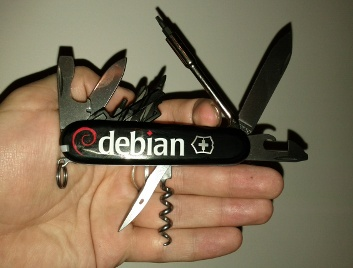
\includegraphics[height=2cm]{../images/debswiss.jpg}
    \end{pgfpicture}
  }
\end{frame}

\subsection{Projects and plans}
\begin{frame}
\frametitle{What are we up to now?}
\begin{itemize}
\item Translation of the free \emph{Debian Administrator's Handbook}, written by Raphael Hertzog and Roland Mas
\item Planning the debian-linux.ro website in order to rebuild a part of it (we recently bought debian.org.ro domain)
\item Organizing meetings!
\item Keep in touch with the community
\end{itemize}
\end{frame}

\begin{frame}
\frametitle{What can we do next?}
\begin{itemize}
\item Workshop.deb (or "how to package stuff for Debian")
\item Installfest
\item Technical meetings with DMs (~MiniDebConf)
\item Bug Squashing Parties
\item Launch parties (\emph{not that hard, they are rare} \smiley )
\end{itemize}
\end{frame}

\begin{frame}
\frametitle{What do we want?}
\begin{itemize}
\item An increased number of 100\% "Made in Romania" contributions
\item Even more Debian Members and Debian Developers
\item Fully, regulated translation of the DPN (\emph{Debian Project News})
\item Increased popularity forthe operating system amongst GNU/Linux users
\end{itemize}
\end{frame}


\section{Final} 
\begin{frame}
\centerline{Questions?}
\end{frame}
% End of slides
\end{document} 